\chapter{散射、对偶性与Veneziano振幅}

\lectureoverview{散射将碰撞约化为可与实验比较的不变量数据。对于四个全同粒子，这些数据可以组织为Mandelstam变量\(s,t,u\)，其中只有两个是独立的。普通的粒子交换于是提示存在分离的直接道与交叉道。Veneziano振幅推翻了这一预期：一个函数同时包含两种道的描述。本讲的后半部分从两条开弦出发构造该函数：它们相接、作为一个振荡链演化，然后再次分裂。}

\section{理论必须预言什么}

费米弦解决了纯玻色模型的两个缺陷：它们允许费米子态，并且在适当的投影之后消除快子。它们的临界时空维数是十而不是二十六。因此额外维度仍然存在，但其紧致化被推迟。当前的主题是散射。
\editorialnote{无快子的陈述指的是在所需投影之后自洽的超弦谱；仅仅加入世界面费米子本身并不足够。}

散射未必是粒子所做的最有趣的事情。它只是实验能够干净地重复的操作。将指定的粒子相互射向对方，记录从碰撞中出射的粒子，并推断隐藏在相互作用区域内部的动力学。当一个理论给出复振幅
\begin{equation}
  \mathcal A(\hbox{incoming data}\to\hbox{outgoing data}),
\end{equation}
时，它才成为定量的；该振幅的模平方与通常的相空间因子一起给出该结果的概率。

\begin{figure}[H]
  \centering
  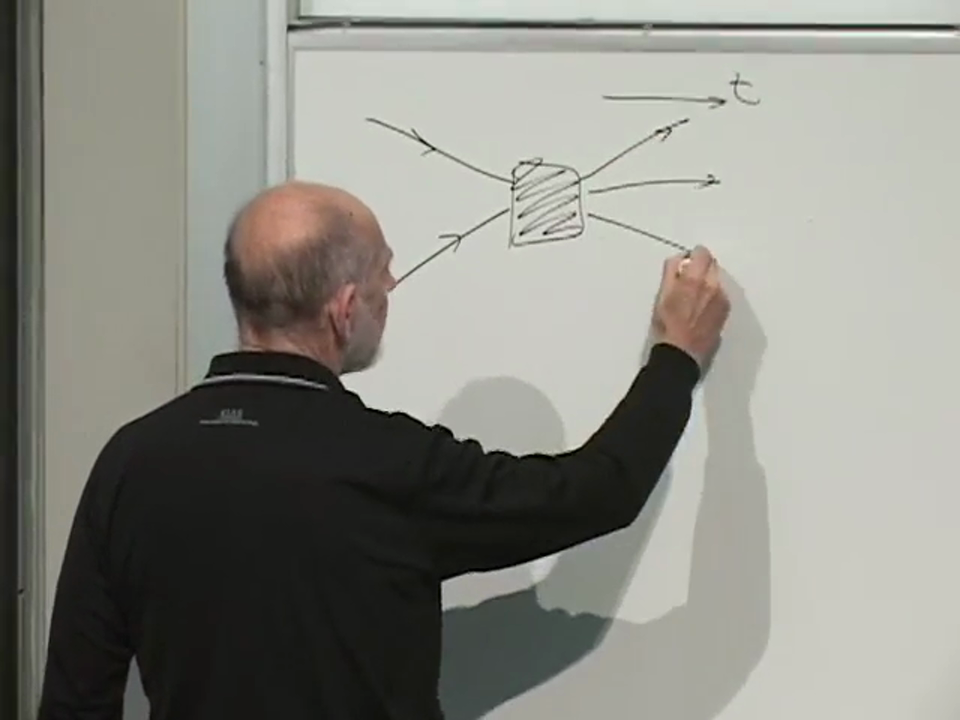
\includegraphics[width=0.72\textwidth]{lecture_06_figure_01.png}
  \caption{入射粒子进入黑箱相互作用区域，出射粒子从中射出；时间水平绘制。}
  \lectureframe{00:02:35}
  \label{fig:l06-black-box}
\end{figure}

粒子还带有自旋、电荷和种类标签。为了首先揭示运动学，让我们暂时抑制除动量以外的一切。

\section{四动量与全入射约定}

将一个粒子的四动量写为
\begin{equation}
  k^\mu=(k^0,\mathbf k)=(E,\mathbf p).
\end{equation}
本讲使用mostly-plus度规，因此
\begin{equation}
  k^2\equiv \mathbf p^2-E^2.
\end{equation}
相对论色散关系因此为
\begin{equation}
  E^2-\mathbf p^2=m^2,
  \qquad
  k^2=-m^2.
  \label{eq:l06-mass-shell}
\end{equation}
改变空间动量会改变能量，但不会使粒子离开其质量壳。

\begin{figure}[H]
  \centering
  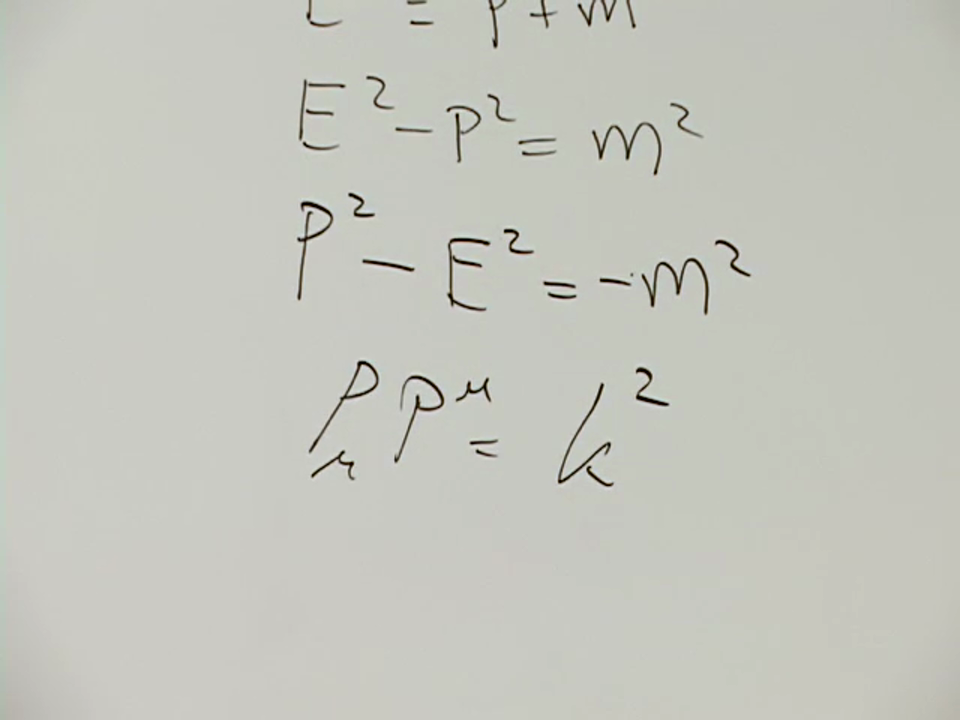
\includegraphics[width=0.66\textwidth]{lecture_06_figure_02.png}
  \caption{本讲通篇所用度规约定下的质量壳条件。}
  \lectureframe{00:05:56}
  \label{fig:l06-mass-shell}
\end{figure}

考虑两个粒子以动量\(k_1,k_2\)入射，两个粒子以物理动量\(q_3,q_4\)出射。能量与动量守恒是一个四矢量方程，
\begin{equation}
  k_1+k_2=q_3+q_4.
  \label{eq:l06-physical-conservation}
\end{equation}
方便的做法是为每条外线指定一个入射动量：
\begin{equation}
  k_3\equiv-q_3,
  \qquad
  k_4\equiv-q_4.
\end{equation}
于是
\begin{equation}
  k_1+k_2+k_3+k_4=0,
  \label{eq:l06-all-incoming}
\end{equation}
并且每条腿都满足\(k_i^2=-m_i^2\)。出射粒子只有在这种记账约定下才具有负能量；它们的物理能量仍然为正。

\begin{figure}[H]
  \centering
  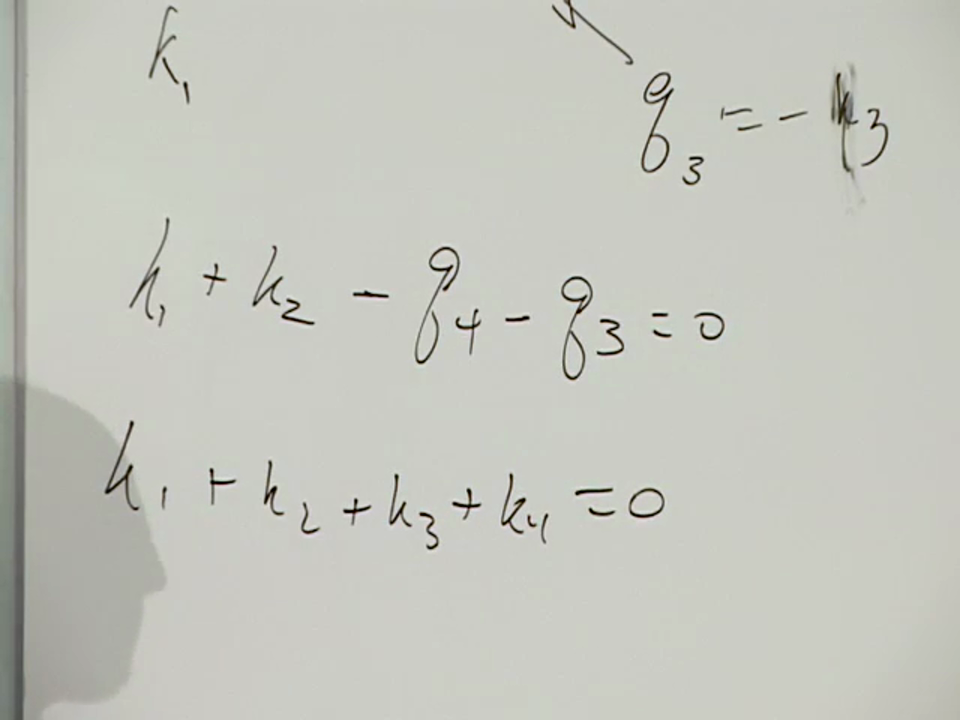
\includegraphics[width=0.68\textwidth]{lecture_06_figure_03.png}
  \caption{物理出射动量被反向，以便所有四个外部动量都可以对称地当作入射来处理。}
  \lectureframe{00:09:10}
  \label{fig:l06-all-incoming-board}
\end{figure}

起初振幅看起来是十六个分量的函数，
\(\mathcal A(k_1,k_2,k_3,k_4)\)。其中大多数是冗余的。转到质心系，将入射动量旋转到选定的轴上，并为了简单起见假设四个粒子质量相同。入射态于是由一个数固定，即质心能量。出射空间动量必须大小相等、方向相反，并且其大小与入射粒子对相同。只剩下它们的偏转角\(\theta\)。因此该过程有两个独立的运动学变量：
\begin{equation}
  E_{\mathrm{cm}},
  \qquad
  \theta.
  \label{eq:l06-two-data}
\end{equation}

\section{Mandelstam变量}

\eqref{eq:l06-two-data}中的两个物理量应当能够不选择参考系地表达。采用全入射约定，定义
\begin{equation}
  \begin{aligned}
    -s&=(k_1+k_2)^2,\\
    -t&=(k_1+k_3)^2,\\
    -u&=(k_1+k_4)^2.
  \end{aligned}
  \label{eq:l06-mandelstam}
\end{equation}
在质心系中，\(k_1+k_2\)的空间部分相消，因此
\begin{equation}
  s=E_{\mathrm{cm}}^2.
  \label{eq:l06-s-energy}
\end{equation}

对于出射物理动量\(q_3=-k_3\)，
\begin{equation}
  k_1+k_3=k_1-q_3
\end{equation}
是从腿1转移到腿3的动量。对于相等的外部质量，设入射空间动量大小为\(p\)，
\begin{equation}
  -t=2p^2(1-\cos\theta),
  \qquad
  -u=2p^2(1+\cos\theta).
  \label{eq:l06-tu-angle}
\end{equation}
因此\(t\)和\(u\)携带探测器所测量的角度信息。

\begin{figure}[H]
  \centering
  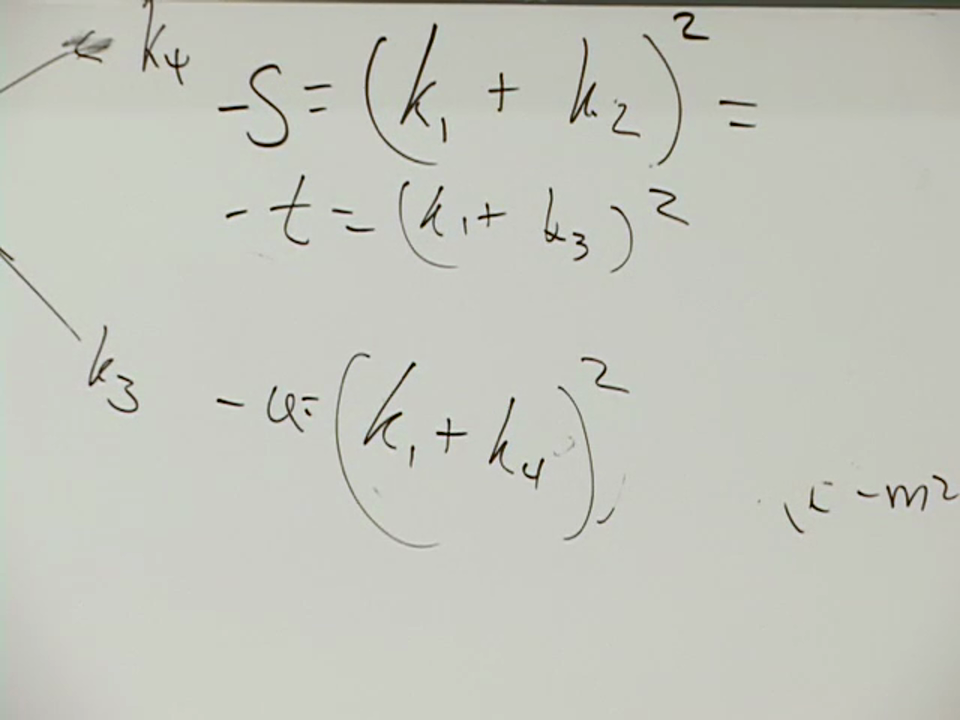
\includegraphics[width=0.74\textwidth]{lecture_06_figure_04.png}
  \caption{全入射约定下\(s,t,u\)的对称定义。}
  \lectureframe{00:26:20}
  \label{fig:l06-stu-board}
\end{figure}

三个符号并不意味着三个独立的数据。将
\eqref{eq:l06-all-incoming}平方并利用\(k_i^2=-m^2\)，对于相等质量给出
\begin{equation}
  s+t+u=4m^2
  \label{eq:l06-stu-constraint}
\end{equation}
一旦\(s\)和\(t\)已知，\(u\)就被固定。

\begin{classroomqa}
\audiencequestion{真空能否像摩擦那样使自由运动的粒子减速？\lecturetimestamp{00:27:17}}
\lecturerresponse{在平移不变的真空里不能。缺失的动量无处可去，因此动量守恒禁止这种摩擦。人们可以设想一种介质或一种不同的真空，它选定了一个优先的静止参考系，但那不是这里所使用的真空。}
\end{classroomqa}

\begin{classroomqa}
\audiencequestion{为什么两个出射粒子必须具有相等的能量？\lecturetimestamp{00:27:54}}
\lecturerresponse{在质心系中，它们的空间动量必须大小相等、方向相反。对于所讨论的等质量过程，相等的动量大小通过\(E^2=p^2+m^2\)给出相等的能量。如果出射粒子的质量不同，那么最后这个结论就必须修改。}
\end{classroomqa}

\section{直接道与交叉道}

一个简单的点粒子图让粒子1和2形成一个质量为\(M\)的中间粒子，该粒子随后衰变为3和4。忽略分子因子和极点规定，其特征依赖关系为
\begin{equation}
  \mathcal A_s\sim\frac{g^2}{s-M^2}.
  \label{eq:l06-s-channel}
\end{equation}
这就是直接过程，或称\(s\)道过程。把连接方式侧转过来，就得到两条外线之间的交换，
\begin{equation}
  \mathcal A_t\sim\frac{g^2}{t-M^2},
  \label{eq:l06-t-channel}
\end{equation}
即交叉过程，或称\(t\)道过程。第三种连接方式给出
\begin{equation}
  \mathcal A_u\sim\frac{g^2}{u-M^2}.
  \label{eq:l06-u-channel}
\end{equation}

\begin{figure}[H]
  \centering
  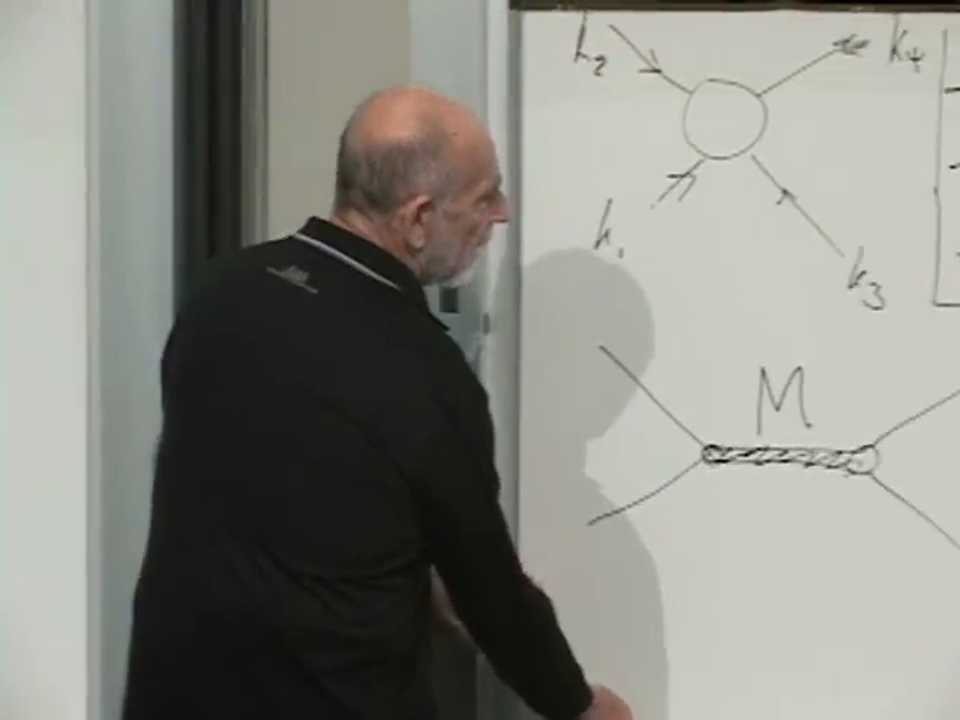
\includegraphics[width=0.72\textwidth]{lecture_06_figure_05.png}
  \caption{通过中间态的直接产生以及相应的极点\(g^2/(s-M^2)\)；交叉连接方式正在同一块黑板上拼装。}
  \lectureframe{00:30:50}
  \label{fig:l06-channel-board}
\end{figure}

这一区别是物理上的。在这个粗糙的标量层面上，\eqref{eq:l06-s-channel}依赖于碰撞能量，但不依赖于角度。复合态在衰变之前已经忘记了入射方向，因此它的衰变是各向同性的。交换振幅依赖于动量转移，因而依赖于角度；轻的交换粒子强烈倾向于小偏转。自旋会带来进一步的角度依赖，但极点结构已经可见。

\begin{classroomqa}
\audiencequestion{缺失的\(u\)道是否产生第三项？\lecturetimestamp{00:34:47}}
\lecturerresponse{是的，只要粒子身份和耦合允许这种连接方式。于是人们就纳入一个在\(u=M^2\)处有极点的项。它不是一个新的独立运动学变量，因为\(s+t+u=4m^2\)，但它是一个不同的道图。}
\end{classroomqa}

\section{一个函数，两种道描述}

单个极点作为介子散射的模型是很差的。两个介子可以形成许多共振态，具有一系列质量和角动量。1960年代的第一反应是添加更多的\(s\)道极点、更多的\(t\)道极点，以及允许的\(u\)道极点。随后人们发现了一个经济得多的函数。在讲座的单位制中，线性雷吉轨迹及其截距已被吸收进\(s\)和\(t\)，该函数为
\begin{equation}
  \mathcal A_{\mathrm V}(s,t)
  \propto
  \frac{\Gamma(-s)\Gamma(-t)}{\Gamma(-s-t)}.
  \label{eq:l06-veneziano}
\end{equation}
伽马函数延拓了阶乘：
\begin{equation}
  \Gamma(n)=(n-1)!
\end{equation}
在正整数处成立。

\begin{figure}[H]
  \centering
  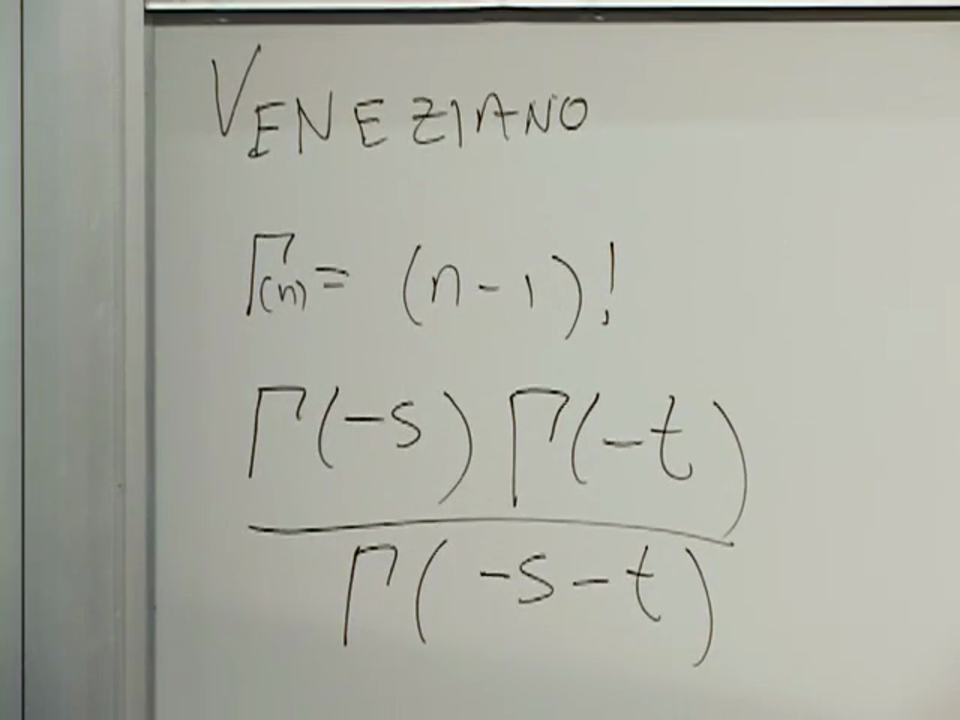
\includegraphics[width=0.68\textwidth]{lecture_06_figure_06.png}
  \caption{写成伽马函数对称比值的韦内齐亚诺振幅。}
  \lectureframe{00:42:25}
  \label{fig:l06-veneziano-board}
\end{figure}

\(\Gamma(-s)\)的极点再现了直接道共振态的无限序列。然而同一个表达式在\(s\leftrightarrow
t\)下是对称的，因此它的\(\Gamma(-t)\)极点给出交叉道展开。这些并不是两个分别添加的贡献。一个解析函数容许两种描述。这就是直接道共振态与交叉道交换之间对偶性的旧观念。

\begin{classroomqa}
\audiencequestion{一个振幅如何能在不把它们相加的情况下同时包含两个道的求和？\lecturetimestamp{00:43:32}}
\lecturerresponse{这正是令人惊讶之处。在\(s\)道极点附近展开该函数，就把它组织为直接共振态；在\(t\)道极点附近展开该函数，就把同一个函数组织为交换。要解释为什么这两种读法是同一回事，需要一个微观模型，而这个模型就是相互作用弦。}
\end{classroomqa}

\section{开弦扫出的一条带}

用下式参数化一条开弦：
\begin{equation}
  0\leq\sigma\leq\pi.
\end{equation}
标记\(\sigma\)不是时空位置。嵌入\(X^\mu(\sigma,\tau)\)告诉我们那个带标记的点位于时空中的何处，而\(\tau\)度量演化。点粒子扫出一条世界线；运动的弦扫出一个二维世界面。在自由理论中，每个嵌入坐标满足
\begin{equation}
  \frac{\partial^2X^\mu}{\partial\tau^2}
  -
  \frac{\partial^2X^\mu}{\partial\sigma^2}
  =0.
  \label{eq:l06-wave-equation}
\end{equation}

\begin{figure}[H]
  \centering
  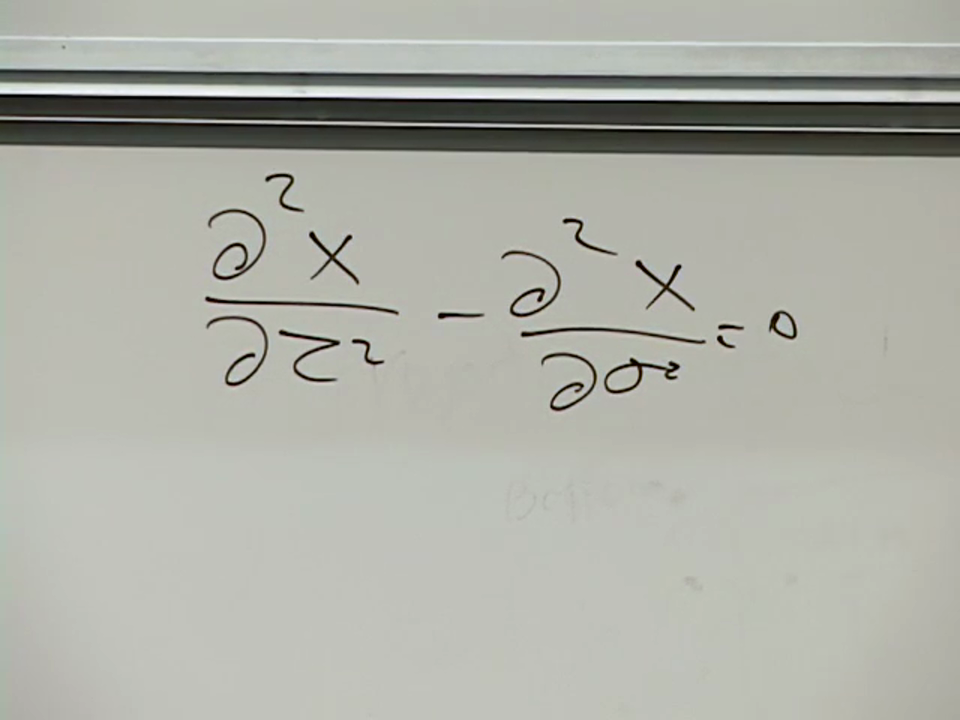
\includegraphics[width=0.70\textwidth]{lecture_06_figure_07.png}
  \caption{支配世界面带上的每个自由弦坐标的波动方程。}
  \lectureframe{00:49:10}
  \label{fig:l06-wave-equation-board}
\end{figure}

对于散射构造而言，不宜过早取连续极限。将每根弦替换为\(n\)个由弹簧连接的质量点。世界面于是成为邻近世界线的一个稠密集合，其简正模就是普通的谐振子。两条入射链可以在其端点处接触。在该事件处，一根新弹簧将它们连接起来，它们作为一根更长的链演化一段时间\(\tau\)，随后一根弹簧断裂，于是两条出射链出现。

\begin{figure}[H]
  \centering
  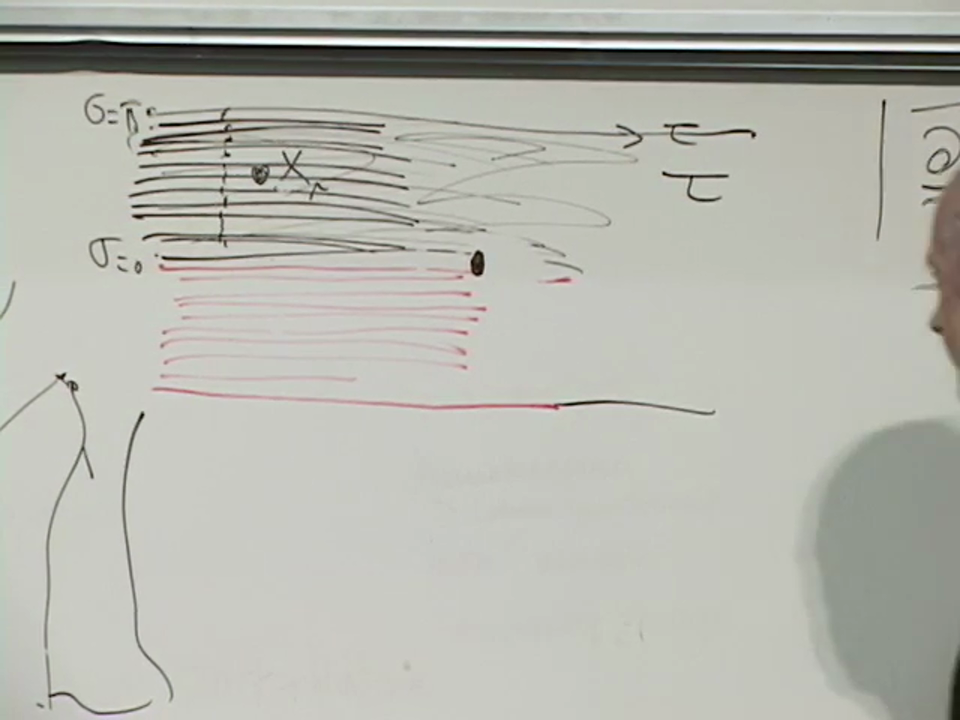
\includegraphics[width=0.72\textwidth]{lecture_06_figure_08.png}
  \medskip

  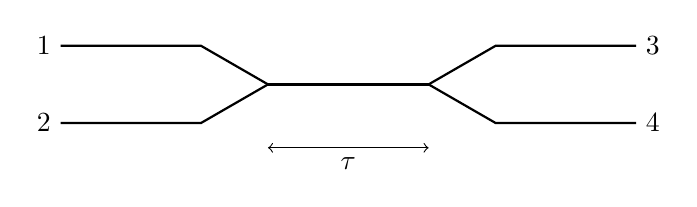
\begin{tikzpicture}[x=0.85cm,y=0.70cm]
    \draw[thick] (0,2.2) -- (2.1,2.2) -- (3.1,1.5);
    \draw[thick] (0,0.8) -- (2.1,0.8) -- (3.1,1.5);
    \draw[thick] (3.1,1.5) -- (5.5,1.5);
    \draw[thick] (5.5,1.5) -- (6.5,2.2) -- (8.6,2.2);
    \draw[thick] (5.5,1.5) -- (6.5,0.8) -- (8.6,0.8);
    \draw[<->] (3.1,0.35) -- node[below] {\(\tau\)} (5.5,0.35);
    \node[left] at (0,2.2) {1};
    \node[left] at (0,0.8) {2};
    \node[right] at (8.6,2.2) {3};
    \node[right] at (8.6,0.8) {4};
  \end{tikzpicture}
  \caption{两条离散化的开弦接触，形成一根中间弦并持续一段时间\(\tau\)，然后分裂。源帧保留了弹簧与世界线的构造；示意图则将其连通性单独抽出。}
  \lectureframe{00:51:25}
  \label{fig:l06-string-joining}
\end{figure}

这两根弦只是在参数空间中被画成相邻。它们的时空位置不必相邻，直到端点坐标真正重合为止。重参数化自由度使得连接与分裂事件可以被放置在图上方便的位置；这一几何自由度将在下一讲中成为共形对称性。

\section{慢动作中的振子计算}

设第一条链的坐标为\(x_1,\ldots,x_n\)，第二条链的坐标为\(x_{n+1},\ldots,x_{2n}\)。它们的质心坐标为
\begin{equation}
  X_{\mathrm{cm}}^{(1)}
  =\frac1n\sum_{a=1}^{n}x_a,
  \qquad
  X_{\mathrm{cm}}^{(2)}
  =\frac1n\sum_{a=n+1}^{2n}x_a.
  \label{eq:l06-chain-centers}
\end{equation}
具有确定动量\(k_1\)的链，其波函数为质心平面波乘以内部振子基态：
\begin{align}
  \Psi_1
  &=
  e^{ik_1\cdot X_{\mathrm{cm}}^{(1)}}
  \psi_0(x_1,\ldots,x_n),
  \\
  \Psi_2
  &=
  e^{ik_2\cdot X_{\mathrm{cm}}^{(2)}}
  \psi_0(x_{n+1},\ldots,x_{2n}).
  \label{eq:l06-two-wavefunctions}
\end{align}
因子\(\psi_0\)依赖于相对坐标，而不依赖于整条链的共同平移。由于入射弦最初是彼此分离的量子系统，
\begin{equation}
  \Psi_{\mathrm{in}}=\Psi_1\Psi_2.
  \label{eq:l06-product-state}
\end{equation}

\begin{figure}[H]
  \centering
  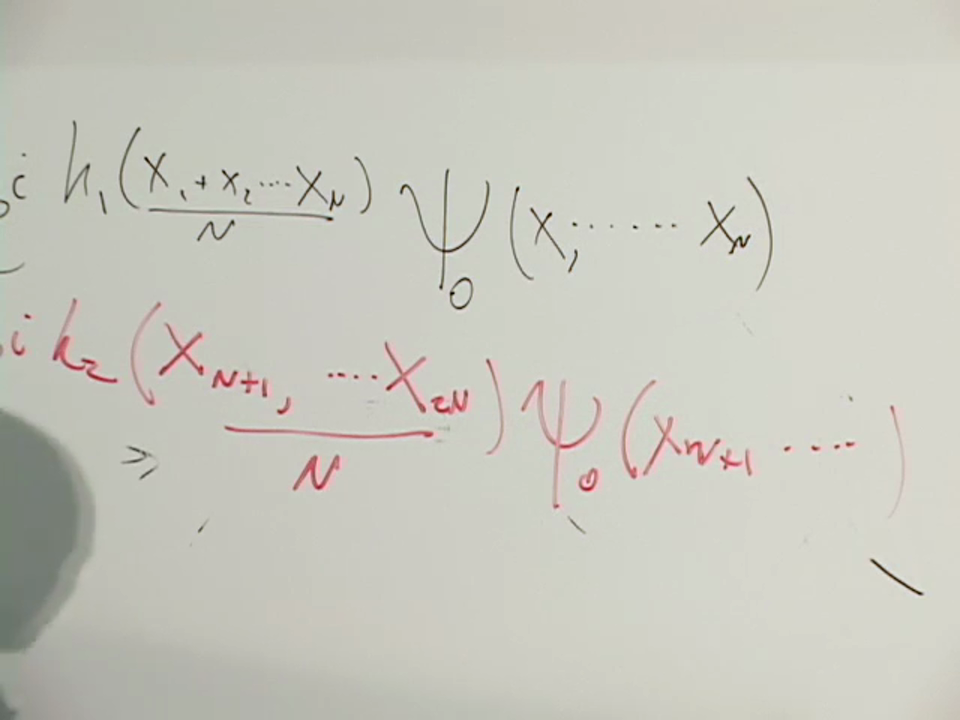
\includegraphics[width=0.76\textwidth]{lecture_06_figure_09.png}
  \caption{两个动量平面波及其内部振子基态因子，以不同颜色写出。}
  \lectureframe{00:58:05}
  \label{fig:l06-wavefunctions-board}
\end{figure}

连接操作选出该波函数中两个端点坐标相一致的部分：
\begin{equation}
  x_n=x_{n+1}.
  \label{eq:l06-endpoint-contact}
\end{equation}
在该瞬间，其余坐标保持不变。随后，所选出的态用单根更长链的哈密顿量\(H_{\mathrm{joined}}\)演化：
\begin{equation}
  \Psi(\tau)
  =
  e^{-iH_{\mathrm{joined}}\tau}\Psi(0).
  \label{eq:l06-time-evolution}
\end{equation}
最后，取它与携带动量\(q_3,q_4\)的出射弦态之积的重叠。

\begin{figure}[H]
  \centering
  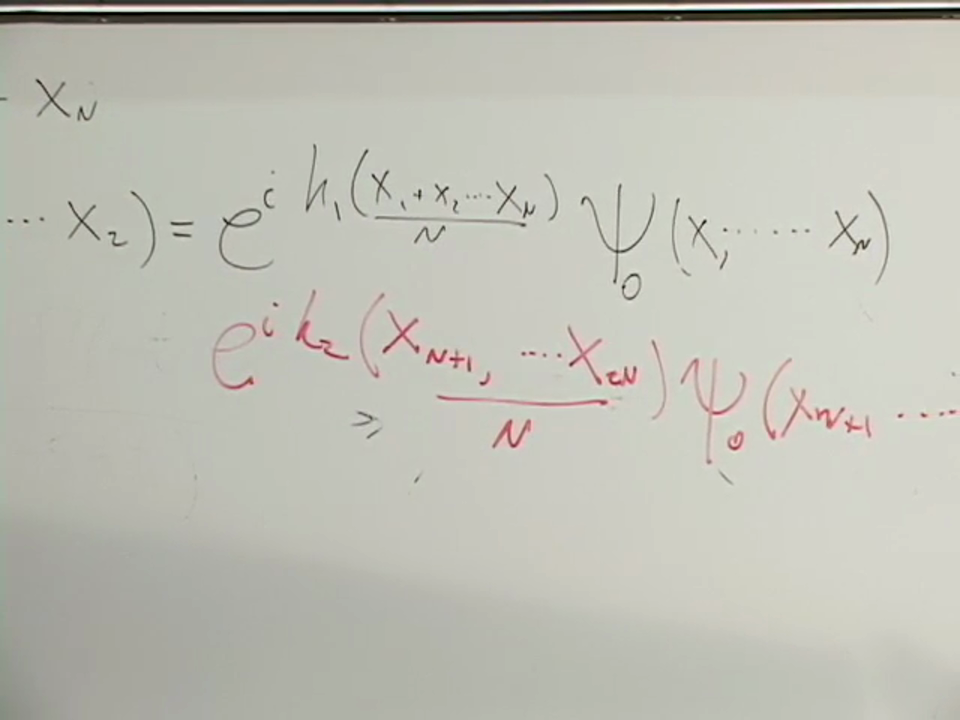
\includegraphics[width=0.76\textwidth]{lecture_06_figure_10.png}
  \caption{在施加端点重合条件之前的两链波函数。}
  \lectureframe{00:58:55}
  \label{fig:l06-endpoint-board}
\end{figure}

计算冗长但并不神秘。每个内部坐标都可以分解为振子模式，因此连接重叠、时间演化和最终投影都归结为高斯振子代数。尚未确定的是连接后弦的寿命\(\tau\)。

\begin{classroomqa}
\audiencequestion{黑色和红色波函数是相加还是相乘？\lecturetimestamp{01:02:26}}
\lecturerresponse{相乘。两个独立系统的张量积态在坐标基下由它们波函数的乘积表示。相加将描述各种备选可能性的叠加，而不是两条入射弦的同时存在。}
\end{classroomqa}

\begin{classroomqa}
\audiencequestion{为什么要对中间时间\(\tau\)积分？\lecturetimestamp{01:04:04}}
\lecturerresponse{连接后的弦并未被赋予固定的寿命。费曼规则是对所有允许的历史求和振幅。在这一描述中，剩余的连续历史参数就是连接与分裂之间的时间，因此求和变为对\(0\leq\tau<\infty\)的积分。}
\end{classroomqa}

\section{从传播时间到贝塔函数}

在计算完振子重叠之后，结果可以整理为
\begin{equation}
  \mathcal A(s,t)
  \propto
  \int_0^\infty d\tau\,
  e^{\tau(s+1)}
  \bigl(1-e^{-\tau}\bigr)^{-t-1}
  e^{-\tau}.
  \label{eq:l06-tau-integral}
\end{equation}
最后的\(e^{-\tau}\)保持可见，因为它是下一步所需的雅可比因子。等价地，第一个和最后一个指数因子合并为\(e^{s\tau}\)。

\begin{figure}[H]
  \centering
  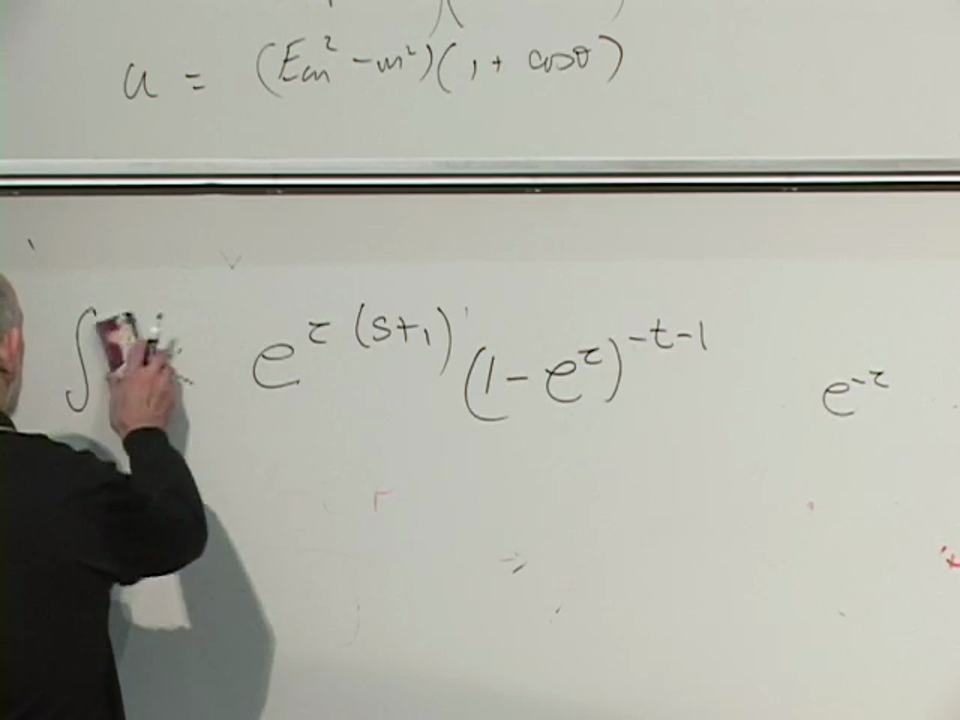
\includegraphics[width=0.76\textwidth]{lecture_06_figure_11.png}
  \caption{振子计算之后的传播时间被积函数；单独的\(e^{-\tau}\)因子提供变量替换的雅可比行列式。}
  \lectureframe{01:06:45}
  \label{fig:l06-tau-integral-board}
\end{figure}

现在令
\begin{equation}
  z=e^{-\tau},
  \qquad
  dz=-e^{-\tau}\,d\tau.
  \label{eq:l06-z-substitution}
\end{equation}
当\(\tau\)从\(0\)变到\(\infty\)时，\(z\)从\(1\)变到\(0\)。负号使积分限反转，得到
\begin{equation}
  \mathcal A(s,t)
  \propto
  \int_0^1
  z^{-s-1}(1-z)^{-t-1}\,dz.
  \label{eq:l06-beta-integral}
\end{equation}

\begin{figure}[H]
  \centering
  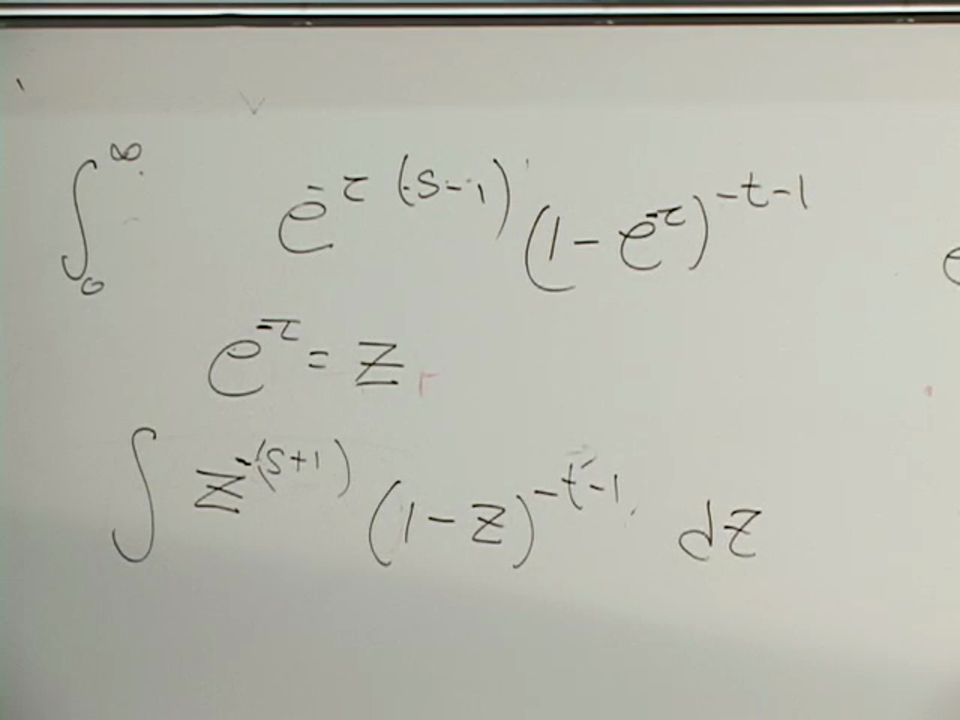
\includegraphics[width=0.74\textwidth]{lecture_06_figure_12.png}
  \caption{代换\(z=e^{-\tau}\)使欧拉贝塔积分显现出来。}
  \lectureframe{01:08:49}
  \label{fig:l06-beta-integral-board}
\end{figure}

该积分在其端点收敛之处直接有定义，在其他地方则由解析延拓定义。它就是欧拉贝塔函数：
\begin{equation}
  B(-s,-t)
  =
  \frac{\Gamma(-s)\Gamma(-t)}{\Gamma(-s-t)}.
  \label{eq:l06-beta-gamma}
\end{equation}

\begin{figure}[H]
  \centering
  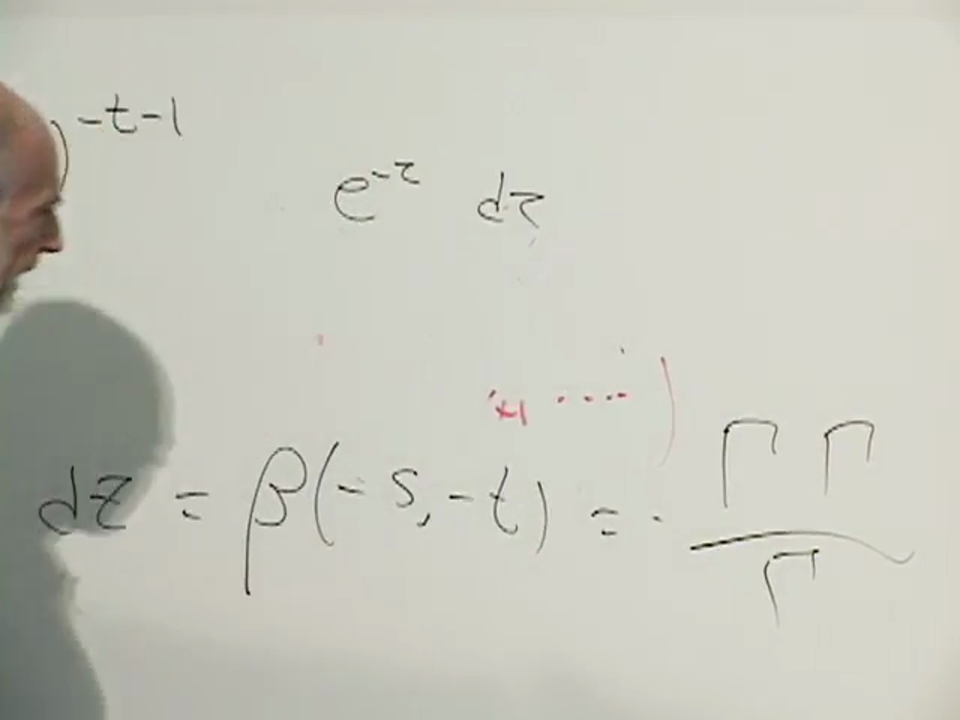
\includegraphics[width=0.72\textwidth]{lecture_06_figure_13.png}
  \caption{黑板上将变换后的积分等同于\(B(-s,-t)\)，并开始恢复其伽马函数形式。}
  \lectureframe{01:12:24}
  \label{fig:l06-beta-gamma-board}
\end{figure}

通道对称性现在是初等的。在\(z\mapsto1-z\)下，
\begin{equation}
  \int_0^1 z^{-s-1}(1-z)^{-t-1}\,dz
  =
  \int_0^1 z^{-t-1}(1-z)^{-s-1}\,dz.
\end{equation}
因此\(\mathcal A(s,t)=\mathcal A(t,s)\)。一个由两条弦连接、随后分裂所构造的过程，自动也包含了交叉描述。
\editorialnote{讲座在贝塔函数的自变量中省略了Regge斜率与截距。在标准记号中，人们把\(s,t\)替换为相应的线性轨迹\(\alpha(s),\alpha(t)\)。对偶性与变量替换论证不变。}

\begin{classroomqa}
\audiencequestion{伽马函数之比类似于组合学中的阶乘表达式。是否存在直接的物理计数解释？\lecturetimestamp{01:13:22}}
\lecturerresponse{在整数自变量处，贝塔函数与诸如\(n!\,m!/(n+m)!\)之比有关，但这里并未断言任何组合机制。同一个特殊函数恰好也来自世界面积分；这一相似性并不是发现该振幅所经由的途径。}
\end{classroomqa}

为什么一个世界面可以在两个通道中被读取，其仍然隐藏的原因是对称性。它允许把面像太妃糖一样拉伸而不改变振幅，从而把长的直接通道传播区域转变为交叉通道交换图像。这一几何解释推迟到下一讲。

\section{散射检验所确立的内容}
\enlargethispage{3\baselineskip}
\begingroup
\setlength{\medskipamount}{3pt plus 1pt minus 1pt}

离散的连接图像引出了最后一组问题。

\begin{classroomqa}
\audiencequestion{如果两条由\(n\)个组分构成的链在其端点处连接，结果是否为\(2n-1\)，并且这会改变费米子宇称吗？\lecturetimestamp{01:16:16}}
\lecturerresponse{在强子端点图像中，相接触的端点对可以被视为一对相互湮灭的粒子-反粒子，因此计数减少二，而不是一。在连续极限下，\(2n\)与\(2n-2\)之间的有限差异无关紧要，但保持费米子宇称并非无关紧要。点阵组分只是连续弦的一个调节器，而不是字面意义上的基本珠子。}
\end{classroomqa}

\begin{classroomqa}
\audiencequestion{后续讨论会继续深入到超弦的完整数学吗？\lecturetimestamp{01:18:05}}
\lecturerresponse{只会用到部分选定的推论。当前的路径是通过世界面对称性和紧致化，随后是1990年代中期发展出的另一个不同出发点：M理论。其目的是从一个视角达到相同的物理，在该视角下若干原本复杂的特征变得透明。}
\end{classroomqa}

\begin{classroomqa}
\audiencequestion{这一连接规则只是来自介子碰撞的一条线索吗？\lecturetimestamp{01:20:02}}
\lecturerresponse{介子散射提供了历史上的线索，但该规则对开弦是普遍的。同样的拓扑描述了开弦光子与其他开弦态的碰撞。两条闭弦通过类似的构造连接与分裂，中间区域有一条闭弦。}
\end{classroomqa}

\begin{classroomqa}
\audiencequestion{该计算是否只在弦态为费米子时适用？\lecturetimestamp{01:20:56}}
\lecturerresponse{不。最初的Veneziano计算属于玻色开弦。超弦需要额外的费米自由度并修改被积函数的细节，但连接、传播、投影以及世界面对偶的逻辑仍然密切类似。}
\end{classroomqa}

在振子谱中发现自旋为一或自旋为二的态是有启发性的，但并非决定性的。它们的散射振幅提供了更强的检验。光子振幅服从与电荷守恒和规范不变性相关的恒等式；引力子振幅服从无质量自旋二场的相应约束。弦态在与有质量和无质量态的相互作用中以及彼此之间的相互作用中通过了这些检验。这就是为什么光子和引力子标签成为物理上的认定，而不是仅基于极化计数的猜测。
\editorialnote{用现代语言来说，这些检验被编码在非物理极化的解耦、规范Ward恒等式以及无质量自旋二态的普适低能耦合中。}

\begin{classroomqa}
\audiencequestion{电荷本身在弦描述中来自何处？\lecturetimestamp{01:24:03}}
\lecturerresponse{这个问题在讲座结束时仍然悬而未决。其答案需要弦理论的内部结构与端点结构，而这些尚未被引入，因此它属于随后的讨论，而不属于这一散射推导。}
\end{classroomqa}
\endgroup
